%
%   Data Analysis
%       - ANOVA and Regression and stuff.
%   
\clearpage
\section{Data analysis}
\label{section:data_analysis}

As stated in our Report's title, the main focus of the analysis will be \textit{Thermal Design Power} and the affect of
other attributes (variables) on this dependent variable.

\textit{Thermal Design Power} \verb|TDP| is an interesting characteristic that comes with the CPU. Theoretically, this is the
maximum amount of heat can be released by its cooling system, which should never be exceeded. This characteristic somehow
represents the heat barrier of a processor, and if its cooling system is designed to deal with almost all the heat it release,
\verb|TDP| roughly equates its power consumption. The higher the \verb|TDP|, the better the CPU's cooling system, but also 
demonstrates the amount of energy consumption required to dissipate the heat.

The reason why we did not use \textit{Temperature} but instead \textit{Thermal Design Power} is that we want to find the amount of
energy needed to keep the CPU operational properly, not the temperature point that CPU can work but be potentially damaged.

We would try to utilize some Regression models to predict its \verb|TDP| via other configurations (or determinants) such as
\textit{Thermal design power}, \textit{Number of cores}, \textit{Base frequency}, \textit{Temperature}, \textit{Lithography},
\textit{Market} and its \textit{Status}. Also, we will see if with the determined \verb|TDP|, we can classify the CPU, whether
it is belong to mass computing devices (Server) or personal usage (Desktop and Mobile).









\subsection{Data preparation}

First, we load the cleaned dataset from the cleaning process above.

\begin{code}{R}
pacman::p_load(
    rio,     # for imports & exports
    ggplot2, # for plots
    zoo      # for year-quarter formats
)

data <- import("cpu-clean.csv") # rio::import
\end{code}

Refer to \textbf{[Figure \ref{fig:hist_tdp}]} and our statement previously, the occurences of values $\ge 150$ is rare, we decided to
cut them out from our dataset. At the same time, we also remove the \mintinline{R}{NAs} rows from the dataset, note that only the
\mintinline{R}{NAs} associated with specific columns are removed, the reason not to remove all is described in \textbf{Section \ref{subsection:data_cleaning}}.

\begin{code}{R}
    data <- data[data$tdp < 150, ]
    data <- data[!is.na(data$tdp), ]
    data <- data[!is.na(data$bfreq), ]
    data <- data[!is.na(data$litho), ]
    data <- data[!is.na(data$ncore), ]
    data <- data[!is.na(data$temp), ]
\end{code}

Because we would make use of Regression models to capture the relationships, a Test Set and a Training Set must be present to perform 
cross-validation to test the fitness of model, besides visualization method by drawing graphs and checking other coefficients. The original
dataset is splitted into two smaller sets, training set and validated set (or test set). In detail, 80\% data is used for training set while 20\% 
is used for test set.

\begin{code}{R}
set.seed(123)

train_indices <- sample(1:nrow(data), nrow(data) * 0.8)
train <- data[train_indices, ]
test <- data[-train_indices, ]
\end{code}

\begin{itemize}
    \item To make to random generation homogeneous among all our tests, we specified a seed (123). Each time we run the cell, we would get
    consistent results of the split.
    \item \verb|sample()| helps us to take a sample from all the elements of our dataset using without replacement. The return value of this function
    are the indices of 80\% the dataset, randomly chosen.
    \item After that, we use simple indexing technique to assign to training set and test set, accordingly.
\end{itemize}











\subsection{The relationships between TDP and other factors}

\subsubsection{The visualizations}
\label{section:data_analysis_visualizations}

\begin{figure}[H]
    \centering
    \begin{subfigure}[b]{0.45\textwidth}
        \centering
        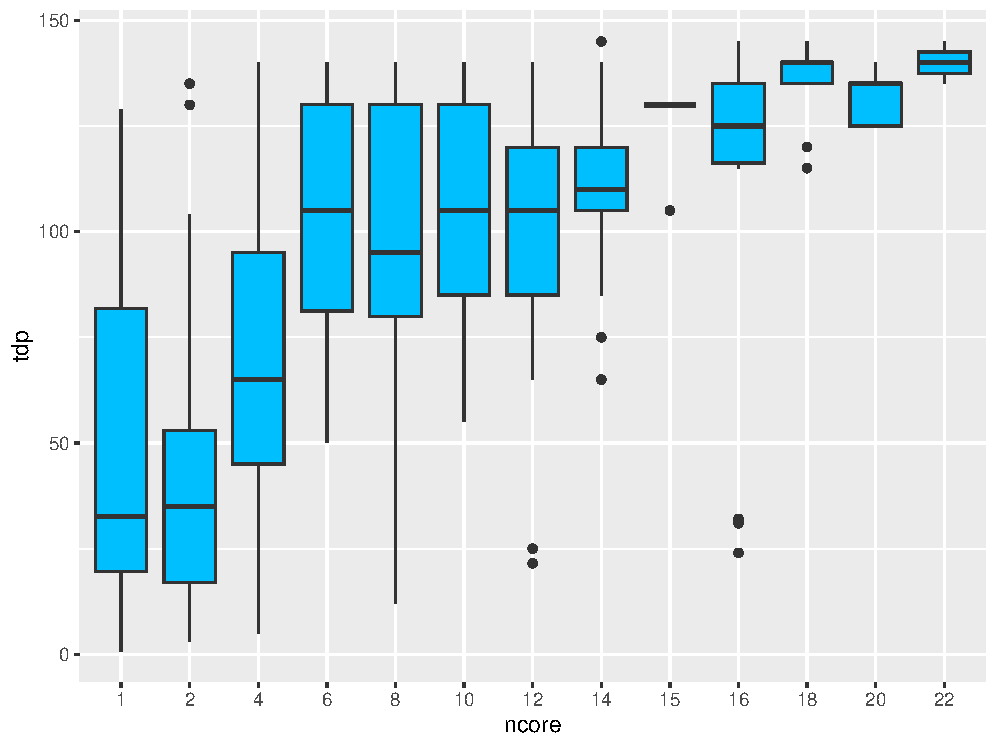
\includegraphics[width=\textwidth]{./graphics/box_tdp_ncore.pdf}
        \caption{Increasing trend of no. cores and TDP}
        \label{fig:tdp_analysis_ncore}
    \end{subfigure}
    \hfill
    \begin{subfigure}[b]{0.45\textwidth}
        \centering
        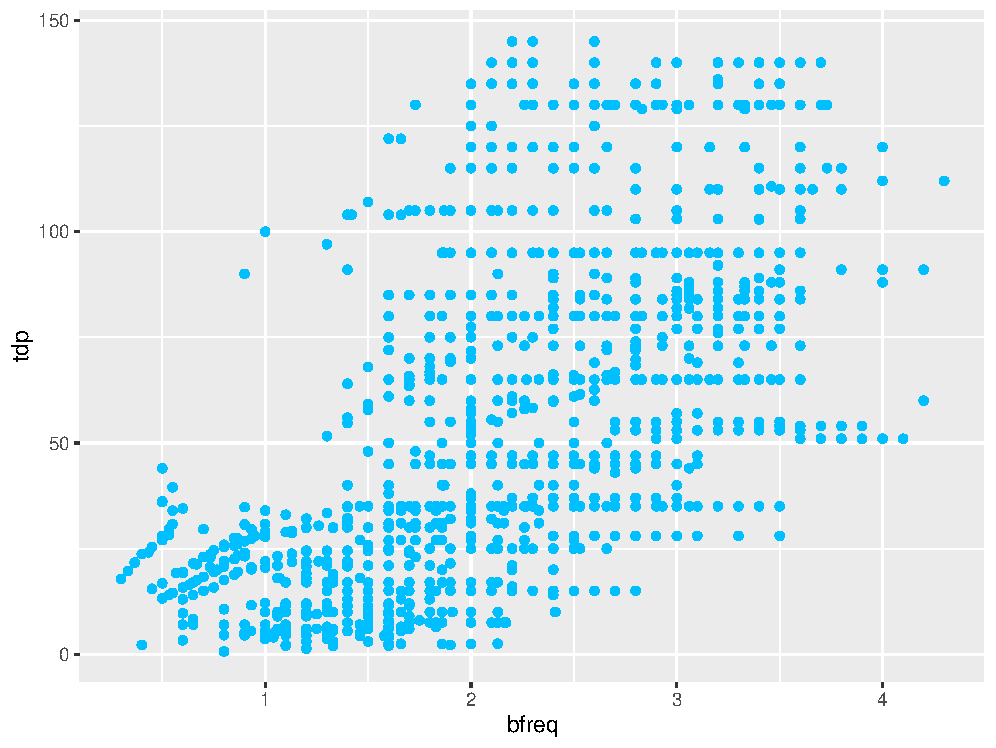
\includegraphics[width=\textwidth]{./graphics/scatter_tdp_bfreq.pdf}
        \caption{Increasing trend of Base frequency and TDP}
        \label{fig:tdp_analysis_bfreq}
    \end{subfigure}
    \hfill
    \begin{subfigure}[b]{0.45\textwidth}
        \centering
        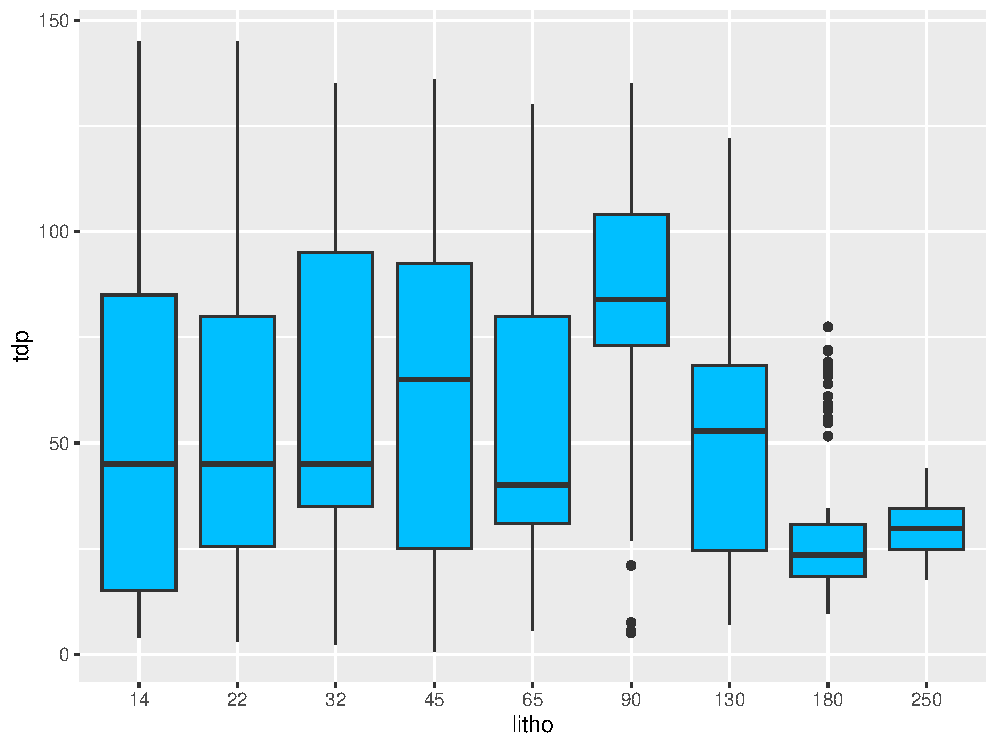
\includegraphics[width=\textwidth]{./graphics/box_tdp_litho.pdf}
        \caption{TDP within different Lithography}
        \label{fig:tdp_analysis_litho}
    \end{subfigure}
    \hfill
    \begin{subfigure}[b]{0.45\textwidth}
        \centering
        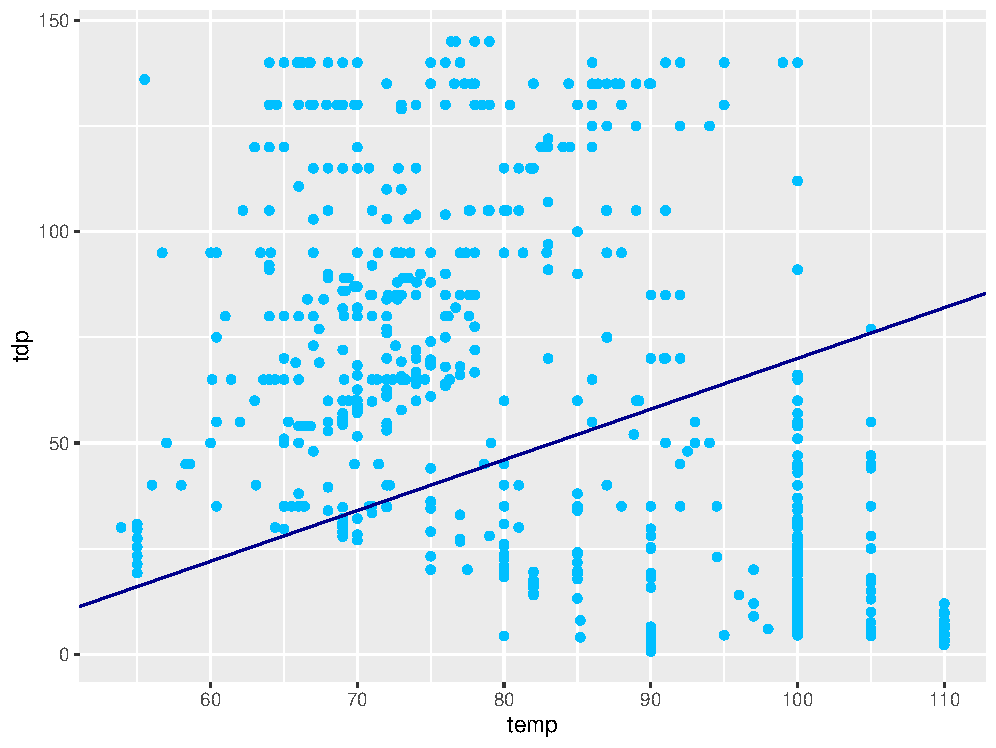
\includegraphics[width=\textwidth]{./graphics/scatter_tdp_temp.pdf}
        \caption{Different trends of TDP on different ranges of temperature}
        \label{fig:tdp_analysis_temp}
    \end{subfigure}
    \hfill
    \begin{subfigure}[b]{0.45\textwidth}
        \centering
        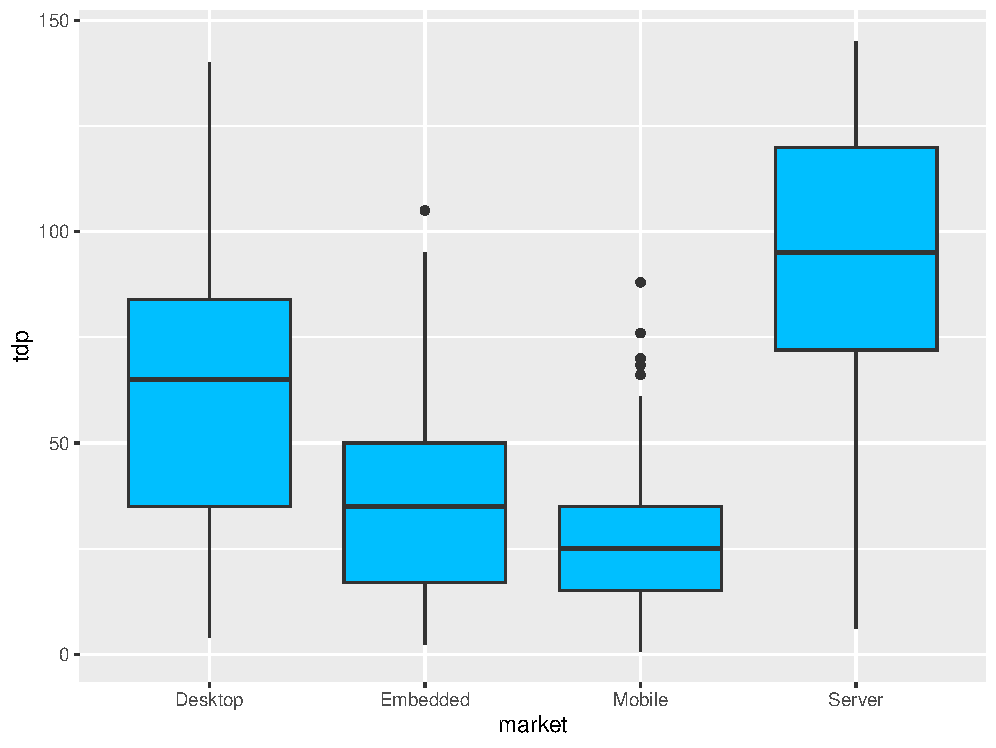
\includegraphics[width=\textwidth]{./graphics/box_tdp_market.pdf}
        \caption{Differences of TDP in different Markets}
        \label{fig:tdp_analysis_market}
    \end{subfigure}

    \caption{The relationship visualizations between TDP and other factors}
    \label{fig:tdp_analysis}
\end{figure}

From the above visualizations, we could make a few comments from these relationships, which motivates us to use certain Regression models:
\begin{itemize}
    \item \textbf{[Figure \ref{fig:tdp_analysis_ncore}]} \verb|tdp ~ ncore| : As \verb|ncore| increases, \verb|TDP| also increases. The variance of \verb|TDP| gets smaller and smaller
    when more and more cores within a CPU appears. This motivates us to with the first Linear regression model (\textbf{Section \ref{section:data_analysis_linear}}).
    However, we also observe that, there was a sharp increase from 1 to 4 cores, then became pretty stable from 6 to 14 cores, then fluctuates wildly for 16 cores
    and above (this argument will be validated in \textbf{Section \ref{section:data_analysis_anova}}). This indicates that Linearity might not be the most desirable
    model, and we need something more powerful to handle such distinctive "clusters" on different ranges, like Random forrest regression
    (\textbf{Section \ref{section:data_analysis_randomforrest}}).
    
    \item \textbf{[Figure \ref{fig:tdp_analysis_bfreq}]} \verb|tdp ~ bfreq| : The data for this relationship is quite variance. However, the dominant trend is still linearly increasing.
    This could be a potential candidate for Linear regression (\textbf{Section \ref{section:data_analysis_linear}}).
    
    \item \textbf{[Figure \ref{fig:tdp_analysis_litho}]} \verb|tdp ~ litho| : There is no clear upward and downward trend for \verb|TDP| as \verb|litho| gets smaller. Instead, we can
    see that \verb|TDP| is converging (\textbf{[Figure \ref{fig:box_litho}]}). Therefore, we can say that \verb|tdp| is getting more and more stable over time.
    And note that, we did say that \verb|litho| is a nice representative of a CPU era instead of \verb|ldate| (thus we said "over time"). This will be explained in further details in 
    \textbf{Section \ref{section:data_analysis_anova}} with visualizations and statistical tests.
    
    \item \textbf{[Figure \ref{fig:tdp_analysis_temp}, \ref{fig:tdp_analysis_market}]} \verb|tdp ~ temp| and \verb|tdp ~ market| : This relationship is interesting. Without the reference line, we can be tempted to conclude that this trend
    is actually heading upward. However, if we take a closer look, there are two different trends happening: above the reference line, we \verb|TDP| actually is increasing and temperature gets higher,
    but the opposite trend occurs for the points below the reference line. In fact, we have a feeling that these two trends come from different market segmentation, so we would plot them out to verify:

        \begin{code}{R}
data$type <- ifelse(data$market == 'Server' | data$market == 'Desktop', "Computers", "Devices")
data$type <- as.factor(data$type)

ggplot(data, aes(x = type, y = tdp)) +
geom_boxplot(fill="deepskyblue")
            
ggplot(data, aes(x = temp, y = tdp)) +
geom_point(color="deepskyblue", ) +
facet_wrap(~data$type)
        \end{code}

        \begin{figure}[H]
            \centering
            \begin{subfigure}[]{0.4\textwidth}
                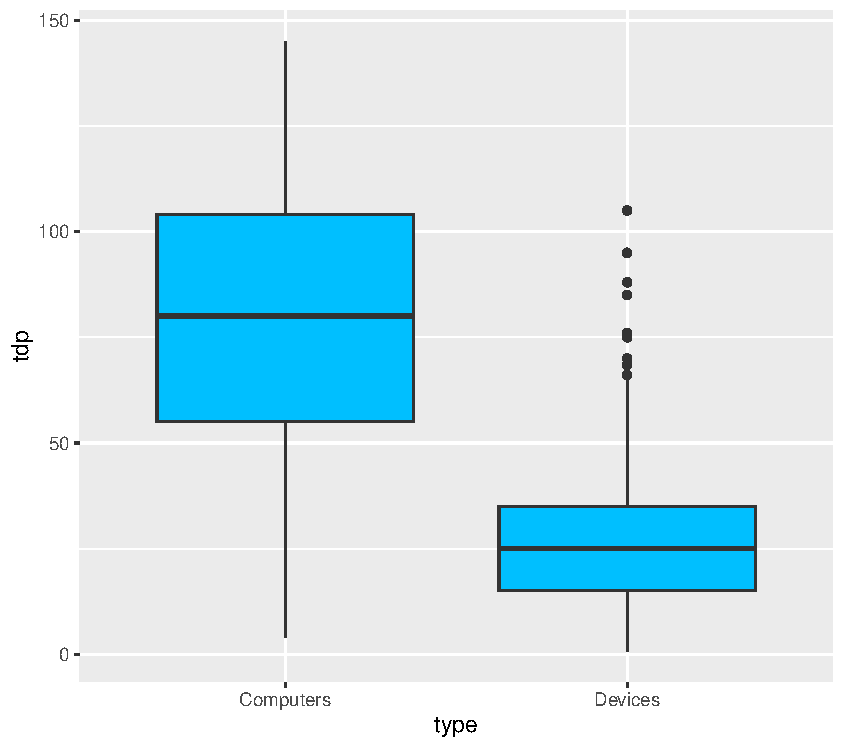
\includegraphics[width=\textwidth]{./graphics/box_tdp_type.pdf}
                \caption{TDP between Types.}
            \end{subfigure}
            \begin{subfigure}[]{0.4\textwidth}
                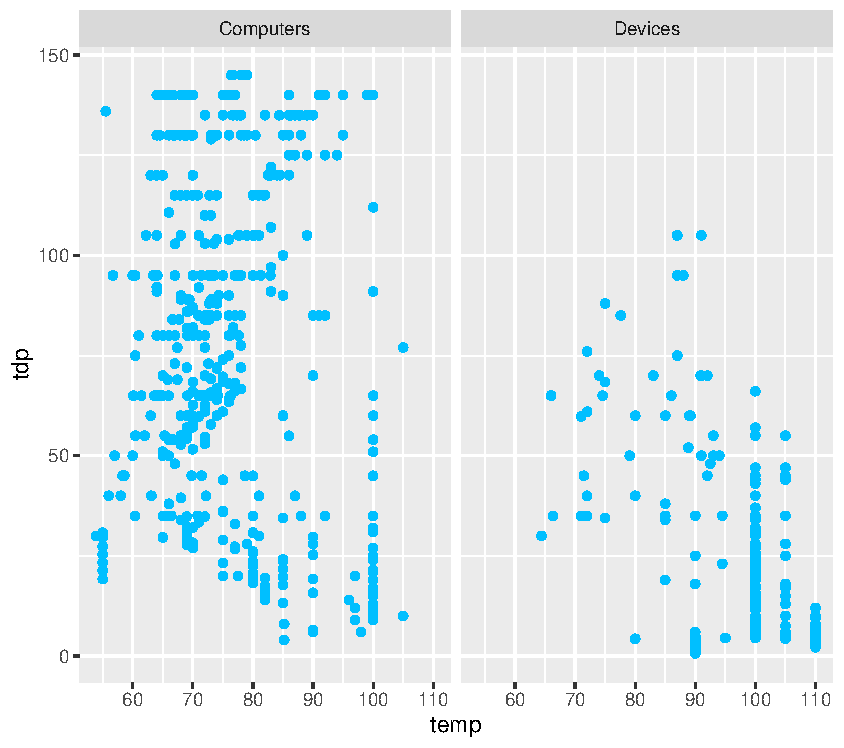
\includegraphics[width=\textwidth]{./graphics/scatter_type_tdp_temp.pdf}
                \caption{TDP in different Market segmentation}
            \end{subfigure}
        \end{figure}

    Turns out, different trends belongs to different Market segmentations (\verb|type|). This could be a potential classfier our data, the idea is to classify \verb|TDP| based on their Market Segmentation first,
    then, we feed the processed data to the Linear regression model or the Random Forrest model to get better performance. Unfortunately, due to the limitation of time and the scope of this assignment, we won't
    go further by using Hybrid models. But this could be a great idea for us for later experiments with an aim to design a better predictor.
\end{itemize}


\subsubsection{Hypothesis testing}
\label{section:data_analysis_anova}

To explain further the statements we made above, we will assess the following assumptions by using several techniques such as 
hypothesis testing, ANOVA and computing the covariances.

The assumptions we are aiming to:
\begin{enumerate}
    \item Lithography as a CPU era.
    \item Thermal Design Power with respect to Number of Cores.
    \item Thermal Design Power with respect to Temperature.
\end{enumerate}











\textbf{Lithography as a CPU era.}

In this small section, we will demonstrate why \textbf{Lithography as a better representative than Launch date}. To do that, we start by looking at the confidence interval and the visualizations of Lithography over the years.

\begin{code}{R}
    data$litho <- as.factor(data$litho)

    retval <- data.frame(NA, NA, NA, NA)
    names(retval)<-c("5% quantile","95% quantile", "STD Mean", "Confidence Interval")
    
    for (lit in levels(data$litho))
    {
          quants <- quantile(
            data[data$litho == lit, ]$ldate,
            na.rm = T,
            probs = c(0.05,0.95)
          )
          
          dates <- data[data$litho == lit, ]$ldate
          
          new_row <- data.frame(quants[1], quants[2], mean(sd(dates, na.rm=TRUE), na.rm=TRUE),quants[2]-quants[1])
          names(new_row)<-c("5% quantile","95% quantile", "STD Mean", "Confidence Interval")
          
          retval <- rbind(retval, new_row)
          rm(dates)
    }
    rownames(retval) <- c("NULL", levels(data$litho))
    retval <- retval[-1,]
    
    print(retval)
    
    ggplot(data, aes(x = ldate, y = litho)) +
      geom_boxplot(fill="deepskyblue")
\end{code}
\begin{figure}[H]
    \centering
    \begin{subfigure}[]{0.5\textwidth}
        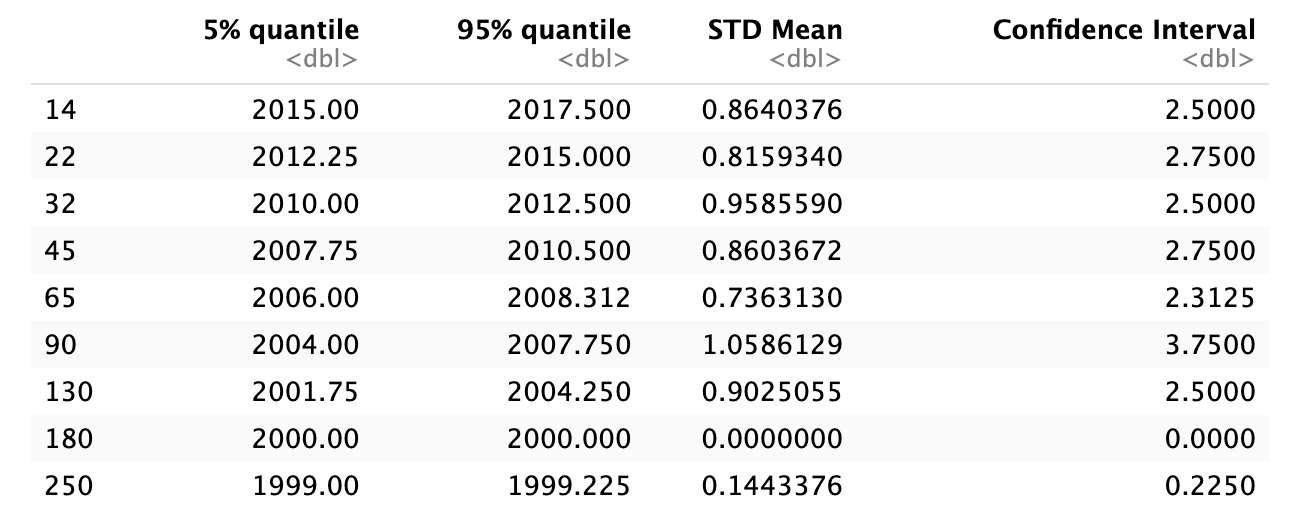
\includegraphics[width=\textwidth]{./graphics/confint_litho.png}
        \caption{Summary of Confidence Interval of Lithography over the years}
    \end{subfigure}
    \begin{subfigure}[]{0.4\textwidth}
        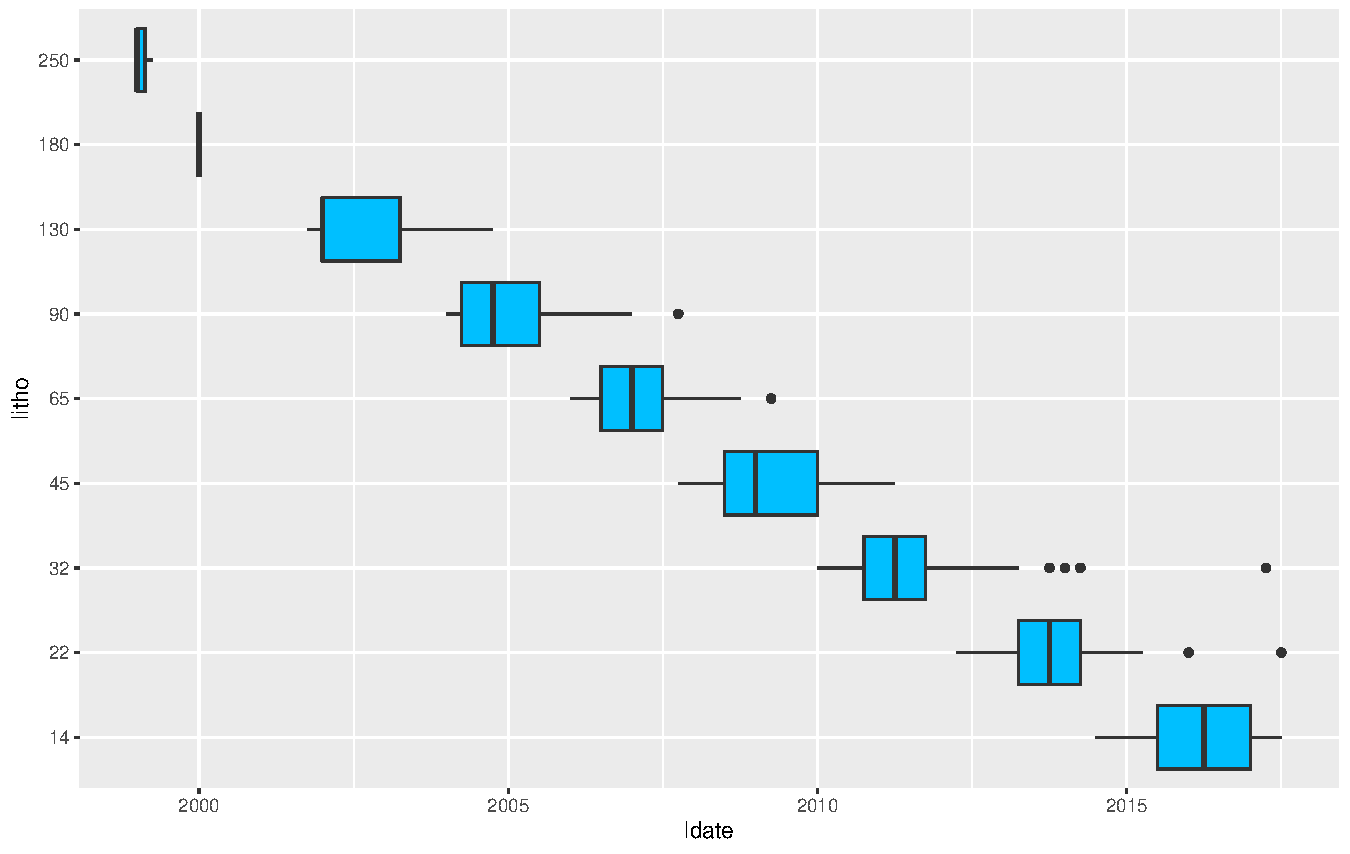
\includegraphics[width=\textwidth]{./graphics/box_ldate_litho.pdf}
        \caption{TDP in different Market segmentation}
    \end{subfigure}
\end{figure}

Looking at the Mean of Standard Deviation (\verb|STD Mean|), these \textit{means are pretty stable}, and the \verb|Confidence Interval| column tells us that
most of the era of CPU design \textit{spans for about two and a half years}, and these era are approximately mutually exclusive. This is its big advantage over
using Launch date only, because we can now consider a range of values and group different launch dates together wich possibly share the same characteristics. So,
everytime we wants to refer to a period of CPU, we always use Lithography.

One more thing we want to emphasize is the \textbf{stability of TDP in recent eras}, and the fact that it is converging. We will test whether this is correct or not using
ANOVA.

We observed that the "stable eras" are when \verb|litho=14,22,32,45,65| \textbf{[Figure \ref{fig:tdp_analysis_litho}]}. They would be taken out and put into an ANOVA model:

\begin{code}{R}
    data_litho_subset <- subset(data, data$litho %in% c(14,22,32,45,65))
    litho_anova_model <- aov(tdp ~ litho ,data = data_litho_subset)
\end{code}
\begin{itemize}
    \item The first line is: Taking any row statisfying its \verb|litho| is 14 or 22 or 32 or 45 or 65.
    \item The second line is: Construct an ANOVA model, with \verb|litho| is categorical variable and \verb|tdp| is explanatory variable.
\end{itemize}

To satisfy the requirements of One-way ANOVA, we should check its assumptions on Normality and Homoscedasticity (homogeneous variance).

\begin{code}{R}
    qqPlot(residuals(litho_anova_model))
    shapiro.test(residuals(litho_anova_model))
    data_litho_subset_clone <- data_litho_subset
    data_litho_subset_clone$litho <- as.factor(data_litho_subset_clone$litho)
    leveneTest(tdp ~ litho ,data = data_litho_subset_clone)
\end{code}
\begin{itemize}
    \item We make a Q-Q Plot to explore its residuals

    \item We perform a Shapiro-Wilk test of Normality:
    
        \qquad Null hypothesis $H_0$ : The residuals of ANOVA model is normally distributed.

        \qquad Alternative hypothesis $H_1$ : The residuals of ANOVA model is not normally distributed.

    \item We create a clone data set to factorize litho, and transforms each lithography into levels.
    
    \item We perform Levene's test to test for the equality of variances.
    
        \qquad Null hypothesis $H_0$ : The variance of \verb|TDP| between categorical \verb|litho| is equal.

        \qquad Alternative hypothesis $H_1$ : The variance between them is not equal.
\end{itemize}
We decided to choose Significant level $\alpha = 0.005$ (since the dataset large, we can choose small $\alpha$, indicating that we are not 
interested in minor differences, which might be significant if the sample size is large), the results 
are displayed as follows:
\begin{figure}[H]
    \centering
    \begin{subfigure}[b]{0.6\textwidth}
        \centering
        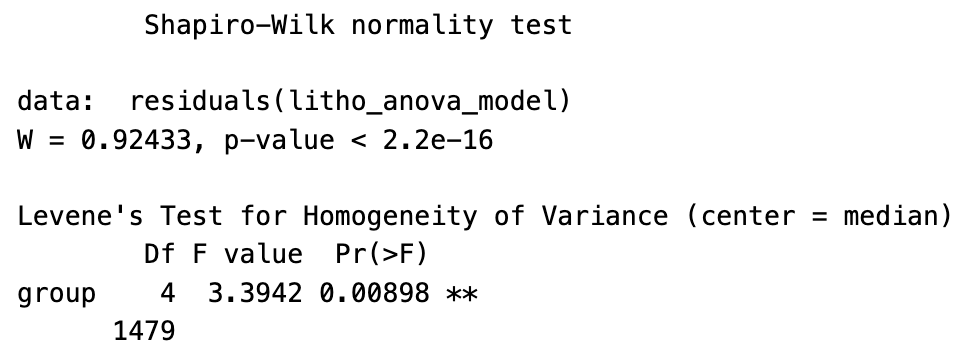
\includegraphics[width=\textwidth]{./graphics/anova_litho_shapiro_wilk.png}
        \caption{Results of Shapiro-Wilk and Levene's Test}
        \label{fig:anova_litho_shapiro_wilk}
    \end{subfigure}
    \begin{subfigure}[b]{0.35\textwidth}
        \centering
        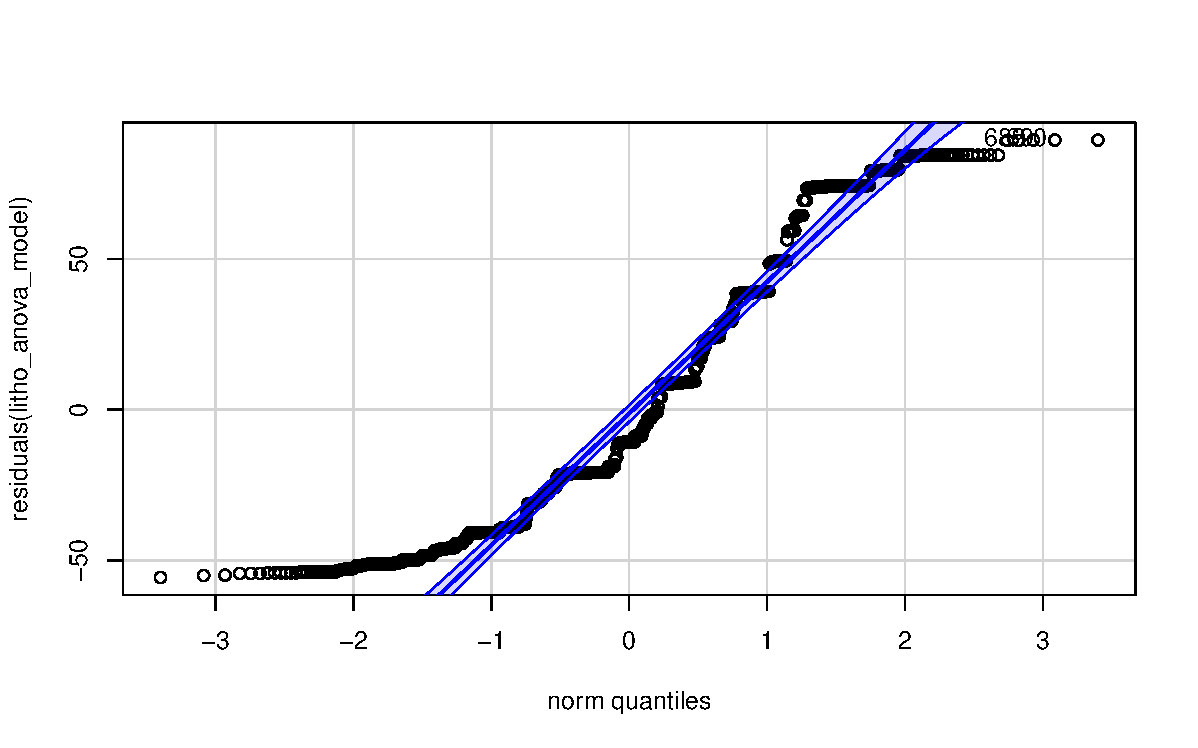
\includegraphics[width=\textwidth]{./graphics/anova_litho_qqplot.pdf}
        \caption{Q-Q Plot of the ANOVA model}
        \label{fig:anova_litho_shapiro_wilk}
    \end{subfigure}
    \caption{Summary of the tests.}
\end{figure}

Variance homogenity test is higher than $\alpha$ (about 0.8\%), infering that there is an apparent
evidence (statistically significant) that the variances are homogeneous. However, the normality assumption is not satisfied, as the Shapiro-Wilk
test failed to keep the Null hypothesis ($p < 2\times10^{-16}$ was so low that it exceeds the capability of calculating in R). The test could have been
not successful since the dataset is large, this is acceptable. However, by looking at the Q-Q plot, we are totally convinced that it is doubtful to
assume the normality of this model. The accuracy of One-way ANOVA might not be reliable.

Because of that, we must utilize a Non-parametric test called Kruskal-Wallis H-Test. This test is robust to non-homogeneous variances, and of course
do not assume the normality of residuals in prior. Also, it can perform on multiple levels. There exists a non-parametric version of One-way ANOVA, 
called Wilcoxon rank-sum test, however this test is only applicable to two levels only.
\begin{itemize}
    \item Kruskal-Wallis H-Test
    
    \qquad Null hypothesis $H_0$ : The \verb|TDP| values of \verb|litho=14,22,32,45,65| come from the same distribution (same median and same variance).

    \qquad Alternative hypothesis $H_1$ : These \verb|TDP| values do not come from the same distribution
\end{itemize}

Choosing $\alpha = 0.05$, we perform the test:
\begin{code}{R}
    kruskal.test(tdp ~ litho, data = data_litho_subset)    
\end{code}

\begin{figure}[H]
    \centering
    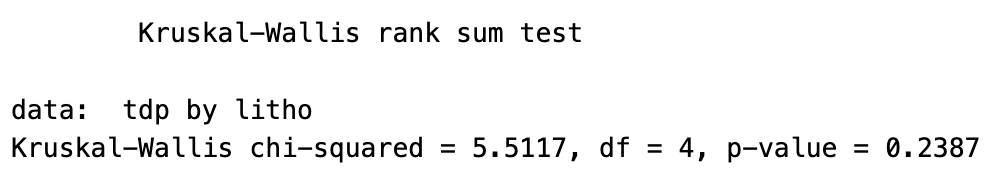
\includegraphics[width=0.5\textwidth]{./graphics/anova_litho_kruskal.png}
    \caption{Summary of Kruskal-Wallis H-Test}
    \label{fig:anova_litho_kruskal}
\end{figure}

The test result of $p$-value is $p = 0.2387 > 0.05$, so we can not reject $H_0$. Therefore, it is not-statistically significant, and they might come
from the same distribution. This test validates the statement we made above. We can conclude that, with \verb|litho| provided, any decision-based model
would perform well categorizing them.









\textbf{Thermal Design Power with respect to Number of Cores}

The relationship of \verb|tdp| and \verb|ncore| is not linear. Let us perform several tests to see it.
    
First, we separate the ncore to some groups.
    
\begin{code}{R}
    group1 <- subset(data, data$ncore %in% c(1,2))
    group3 <- subset(data, data$ncore %in% c(6,8,10,12,14))
    group4 <- subset(data, data$ncore %in% c(15,16,18,20,22))
\end{code}

    By plotting Q-Q plot, we observe that the distribution of residuals is not normal.

\begin{code}{R}
    library(car)
    model<- aov(tdp ~ ncore ,data = group1)
    qqPlot(residuals(model))
\end{code}

\begin{figure}[H]
    \centering
    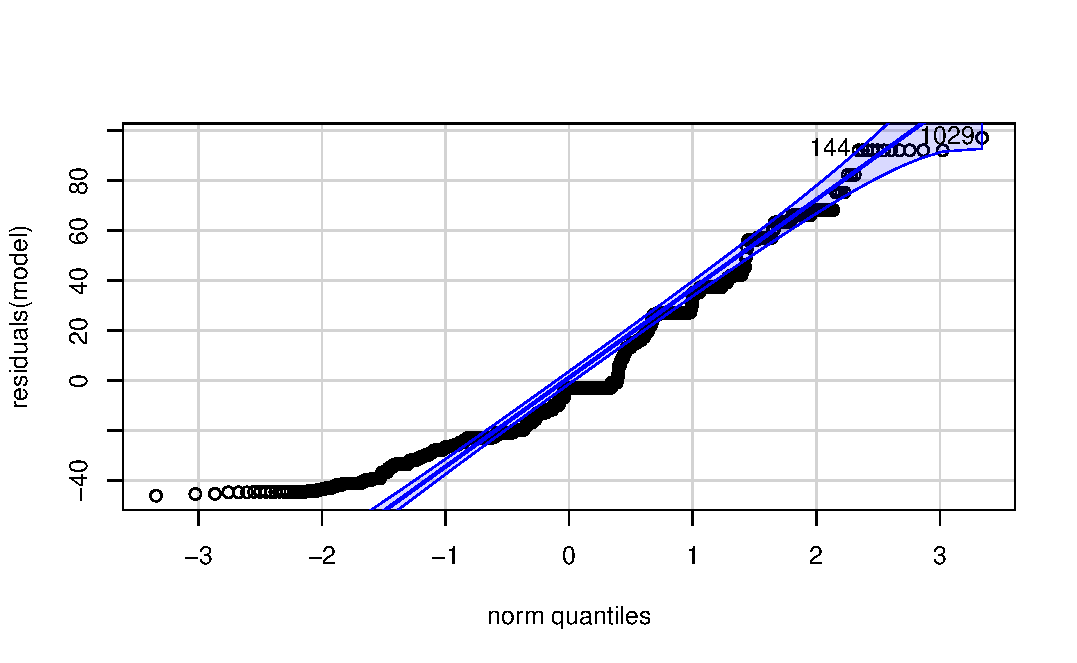
\includegraphics[width=0.5\textwidth]{./graphics/anova_ncore_qqplot.pdf}
    \caption{Q-Q plot of Number of Cores ANOVA model}
    \label{fig:anova_ncore_qqplot}
\end{figure}

    For the same reason of normality, we perform Kruskal-Wallis H-Tests on different intervals:

\begin{code}{R}
    kruskal.test(tdp ~ ncore, data = group1) 
    kruskal.test(tdp ~ ncore, data = group3)
    kruskal.test(tdp ~ ncore, data = group4)
\end{code}

\begin{figure}[H]
    \centering
    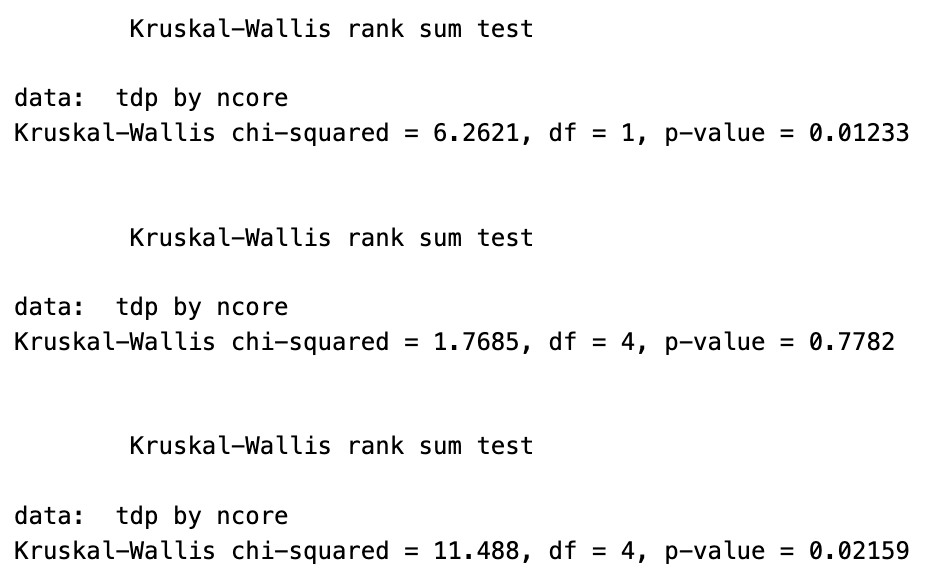
\includegraphics[width=0.5\textwidth]{./graphics/anova_ncore_test.png}
    \caption{Q-Q plot of Temprature model}
    \label{fig:anova_ncore_test}
\end{figure}

We see that the results varies wildly among the intervals. There is an interval which is likely homogeneous, while two other intervals are not.
This means that we do not really have a linear relationship among all the intervals of \verb|ncore|, although on the big picture, it is acceptable.









\textbf{Thermal Design Power with respect to Temperature}

Too really believe there are two trends of \verb|TDP| going on within \verb|temp|, we may want to split the \verb|temp| into
two halves, one for \verb|temp < 85|, and one for \verb|temp >= 85|. Then we will compute the covariance too see if they are really
different.

\begin{itemize}
    \item If the covariance is positive, the trend is likely to go upward,
    \item If the covariance is negative, the trend is likely to go downward.
\end{itemize}

\begin{code}{R}
    group1 <- data[data$temp < 85, ]
    group2 <- data[data$temp >= 85, ]

    cov(group1$tdp, group1$temp)
    cov(group2$tdp, group2$temp)
\end{code}

The results are as follows:
\begin{figure}[H]
    \centering
    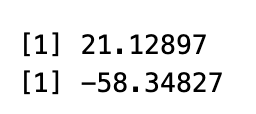
\includegraphics[width=0.5\textwidth]{./graphics/anova_temp_cov.png}
    \caption{Q-Q plot of Temprature model}
    \label{fig:anova_temp_cov}
\end{figure}

Two covariances are different from each other, meaning that there are two different trends going on.
























\subsection{Multiple Linear Regression Model}
\label{section:data_analysis_linear}

We attempt to capture the relationships by using a Linear Regression model. Based on the plots provided in \textbf{Section \ref{section:data_analysis_visualizations}}, 
we have evidence too believe that a Multiple Linear Regression model would perform acceptably in predicting \verb|TDP| based on other factors.

First, we construct the model and plot some figures to check if Normality and Homoscedasticity are satisfied or not:

\begin{code}{R}
model.lr <- lm(tdp ~ ncore + bfreq + litho + temp, data = train) 

# Test for Normality
# and homoscedasticity
ggplot(model.lr, aes(x = resid(model.lr))) +
  geom_histogram(binwidth = 2, fill="deepskyblue") # histogram of residuals
ggplot(model.lr, aes(sample = rstandard(model.lr))) +
  stat_qq(shape=1, color="blue") + stat_qq_line() +
  labs(x="Theoretical quantiles", y="Standardized residuals")

# Summary of the model
summary(model.lr)
\end{code}
\begin{itemize}
    \item The first line in constructing the model. \verb|ncore|, \verb|bfreq|, \verb|litho| and \verb|temp| were used. The coefficients are tuned (or trained) based on \verb|train| 
    data frame we splitted earlier.

    \item The following lines are for plotting the histogram of residuals and standardized Q-Q plot.
    
    \item The last line prints the summary of the model.
\end{itemize}
\begin{figure}[H]
    \centering
    \begin{subfigure}[b]{0.49\textwidth}
        \centering
        \includegraphics[width=\textwidth]{./graphics/linear_reg_hist.pdf}
        \caption{Histogram of residuals}
    \end{subfigure}
    \hfill
    \begin{subfigure}[b]{0.49\textwidth}
        \centering
        \includegraphics[width=\textwidth]{./graphics/linear_reg_qq.pdf}
        \caption{Q-Q Plot of residuals}
    \end{subfigure}
\end{figure}
\begin{figure}[H]
    \centering
    \includegraphics[width=0.5\textwidth]{./graphics/linear_reg_summary.png}
    \label{fig:linear_reg_summary}
\end{figure}
There are some statements that can be concluded from the model summary:
\begin{itemize}
    \item 
\end{itemize}















\subsection{Random Forrest Regression Model}
\label{section:data_analysis_randomforrest}









\subsection{Logistic Regression Model}
\label{section:data_analysis_logistic}